%\usepackage[T1]{fontenc}
%\usepackage[utf8]{inputenc}

%!TEX ROOT=../diploma-thesis.tex

\chapter{Testování a validace frameworku}\label{ch:testovani}

Tato kapitola popisuje, jak\'ym způsobem bylo provedeno
testování naprogramovan\'ych knihoven.
Kapitola se dále věnuje popisu ukázkového systému, na kterém
byla demonstrována správná funkčnost navrženého frameworku
a provedena analýza vlivu jeho nasazení na duplikaci
byznysových pravidel.

\section{Techniky testování}

Pro testování prototypů knihoven bylo využito několik technik testování,
které pomáhají odhalit chyby a zvýšit kvalitu výsledného software.

\subsection{Jednotkové testy}

Jednotkové testy jsou nejnižší úrovní testování, která má za úkol ověřit správnou
funkčnost dílčích částí systémů -- tzv. \textit{jednotek}. Tato technika se
soustředí na odhalení chyb v implementaci dané jednotky.
Jednotkové testy umožňují odhalit chyby v dřívějších fázích vývoje~\cite{luo2001software}.
Usnadňují také následnou integraci jednotek, při které lze využít předpokladu, že jednotky fungují
správně.

\subsection{Integrační testy}

Integrační testy ověřují správnou spolupráci jednotlivých komponent programu a mají za úkol
odhalit chyby v jejich komunikaci a nekonzistence v jejich rozhraních. Existuje více
strategií integračního testování. Při integraci lze inkrementálně postupovat od implementovaných
jednotek směrem k celku, tzv. \textit{bottom-up}, nebo směrem od celku k jednotkám, tzv.
\textit{top-down}, kdy je chování dosud neimplementovaných jednotek simulováno~\cite{graham2008foundations}.
Integrovat lze i celý systém najednou, tato metoda se nazývá \textit{big-bang}. V tomto případě je ale těžké
detekovat původ nalezených chyb.

\subsection{Systémové testy}

Systémové testy mají za úkol ověřit, že výsledný program splňuje specifikaci a funguje jako celek.
Tato metoda se věnuje jak funkčním, tak nefunkčním vlastnostem software~\cite{graham2008foundations}.
Systémové testy patří narozdíl od výše uvedených technik do kategorie \textit{black-box}, tzn. neznají
vnitřní strukturu testovaného programu.

\subsection{Průběžná integrace}

Průběžná integrace (z anglického \textit{continuous integration} -- \gls{CI})~\cite{fowler2006continuous}
slouží k urychlení nalezení defektů software ve fázi vývoje. Nové verze zdrojového kódu jsou do projektu pravidelně
integrovány v krátkých časových intervalech a jejich funkčnost je ověřována automatickými testy. K tomu je
zpravidla využíván tzv. \textit{integrační server}, na kterém jsou testy spouštěny. Díky \gls{CI} je
sn\'{\i}žena pravděpodobnost regrese a dlouhodobě zv\'yšena celková kvalita kódu.

\section{Testován\'{\i} prototypů knihoven}

Prototypy knihoven, jejichž implementace je popsána v kapitole~\ref{ch:implementace},
byly důkladně otestovány pomoc\'{\i} sady jednotkov\'ych a integračn\'{\i}ch
testů a t\'{\i}m byla ověřena jejich správná funkcionalita. Způsob
testován\'{\i} knihoven je popsán zvlášť pro každou platformu. Jako systémový test pak
sloužil ukázkový příklad, který je popsaný v následující sekci~\ref{sec:casestudy}.

V rámci \gls{CI} byl kód knihoven po celou dobu v\'yvoje verzován systémem
Git\footnote{\url{https://git-scm.com/}}, zas\'{\i}lán do centráln\'{\i}ho repozitáře a
s pomoc\'{\i} nástroje Travis \gls{CI}\footnote{\url{https://travis-ci.org/}}
bylo automaticky spouštěno jeho sestaven\'{\i} a testován\'{\i}.
Tento nástroj zároveň vývojáře okamžitě informoval o v\'ysledc\'{\i}ch tohoto procesu.

\subsection{Testovací scénáře}

Každá z knihoven byla testována stejnou sadou testovacích scénářů, skládající se z
jednotkových i integračních testů. Scénáře jsou shrnuty v tabulce~\ref{tbl:test-cases}.
K implementaci a vyhodnocení testů byly pro jednotlivé knihovny použity různé technologie,
které jsou popsány v následujícím textu.

\begin{table}
    \centering
    \begin{tabular*}{\textwidth}{ l l }
        \hline
        \textbf{\#} & \textbf{Popis} \\ \hline \hline
        \textbf{TC01} & \makecell[l]{Pouze identifikátor byznysového kontextu obsahující alfanumerický prefix \\ a název je validní} \\ \hline
        \textbf{TC02} & \makecell[l]{Precondition weaver zkontroluje všechny preconditions vztahující se \\ k aktuálnímu kontextu} \\ \hline
        \textbf{TC03} & \makecell[l]{Precondition weaver nevyhodí výjimku, pokud jsou všechny preconditions \\ splněny} \\ \hline
        \textbf{TC04} & \makecell[l]{Precondition weaver vyhodí výjimku, pokud alespoň jedna precondition \\ není splněna} \\ \hline
        \textbf{TC05} & \makecell[l]{Post-condition weaver aplikuje všechny post-conditions vztahující se \\ k aktuálnímu kontextu} \\ \hline
        \textbf{TC06} & Post-condition weaver správně filtruje atribut objektu \\ \hline
        \textbf{TC07} & Post-condition weaver správně filtruje pole hodnot \\ \hline
        \textbf{TC08} & Post-condition weaver správně filtruje atributy objektů v poli \\ \hline
        \textbf{TC09} & Logický výraz \code{And} odpovídá logické konjunkci \\ \hline
        \textbf{TC10} & Logický výraz \code{Equals} odpovídá logické ekvivalenci \\ \hline
        \textbf{TC11} & Logický výraz \code{Negate} odpovídá logické negaci \\ \hline
        \textbf{TC12} & Logický výraz \code{Or} odpovídá logické disjunkci \\ \hline
        \textbf{TC13} & \makecell[l]{Výraz \code{Constant} správně doplňuje do pravidla konstantu} \\ \hline
        \textbf{TC14} & \makecell[l]{Výraz \code{FunctionCall} správně volá externí funkci} \\ \hline
        \textbf{TC15} & \makecell[l]{Výraz \code{IsNotNull} správně kontroluje, zda v jeho argumentu není prázdný výraz} \\ \hline
        \textbf{TC16} & \makecell[l]{Výraz \code{IsNotBlank} správně kontroluje, zda v jeho argumentu není prázdný \\ řetězec} \\ \hline
        \textbf{TC17} & \makecell[l]{Výraz \code{ObjectPropertyReference} správně vkládá do výrazu hodnotu atributu \\ objektu z kontextu} \\ \hline
        \textbf{TC18} & \makecell[l]{Výraz \code{VariableReference} správně vkládá do výrazu hodnotu proměnné \\ z kontextu} \\ \hline
        \textbf{TC19} & \makecell[l]{Byznysové kontexty jsou korektně inicializovány, jejich závislosti staženy \\ a spojeny} \\ \hline
        \textbf{TC20} & Byznysové kontexty jsou správně a kompletně přenášeny mezi službami \\ \hline
        \textbf{TC21} & Při dokončení transakce se správně uloží upravené i nové byznysové kontexty \\ \hline
        \textbf{TC21} & Při zrušení transakce se neuloží upravené ani nové byznysové kontexty \\ \hline
        \textbf{TC22} & Spouštění byznysových operací je pozastaveno při probíhající transakci \\ \hline
        \textbf{TC23} & Byznysové kontexty jsou správně deserializovány z \gls{XML} \\ \hline
        \textbf{TC24} & Byznysové kontexty jsou správně serializovány do \gls{XML} \\ \hline
        \hline
    \end{tabular*}
    \caption{Testovací scénáře prototypů knihoven}
    \label{tbl:test-cases}
\end{table}

\subsection{Platforma Java}

Prototyp knihovny pro platformu jazyka Java byl testován pomoc\'{\i}
nástroje JUnit\footnote{\url{https://junit.org/junit4/}}, kter\'y poskytuje veškerou potřebnou funkcionalitu pro
jednotkové i integračn\'{\i} testován\'{\i}. Všechny testy byly spouštěny automaticky
při sestavován\'{\i} knihovny pomoc\'{\i} nástroje Maven\footnote{\url{https://maven.apache.org/}}.

\lstinputlisting[
caption={Jednotkový test knihovny pro jazyk Java s využit\'{\i}m nástroje JUnit 4},
label={lst:java-testing},
language=Java,
%frame=single,
]
{code/test_example.java}

Ve zdrojovém kódu~\ref{lst:java-testing} je znázorněn jednotkov\'y test
tř\'{\i}dy \code{BusinessContextWeaver} odpovídající testovacímu scénáři \textit{TC06}, konkrétně
filtrování pole \code{email} objektu \code{user}. Anotace \code{@Test} metody \code{test()} znač\'{\i},
že metoda obsahuje \textit{test case} a framework JUnit zajist\'{\i}, že bude spuštěna
a vyhodnocena. Statické metody tř\'{\i}dy \code{Assert} ověř\'{\i}, zda uživateli zůstalo
vyplněno jméno, ale emailová adresa ne.

\subsection{Platforma Python}

Prototyp knihovny pro platformu jazyka Python byl testován pomoc\'{\i}
nástroje \code{unittest}\footnote{\url{https://docs.python.org/3/library/unittest.html}}, inspirovaného nástrojem
JUnit. Ačkoliv jméno obou nástrojů nasvědčuje, že slouž\'{\i} zejména pro jednotkové testy,
lze je plně využ\'{\i}t i pro integračn\'{\i} testy.

\lstinputlisting[
caption={Jednotkový test knihovny pro jazyk Python s využit\'{\i}m nástroje Unittest},
label={lst:python-testing},
language=Python,
%frame=single,
]
{code/test_example.py}

Ve zdrojovém kódu~\ref{lst:python-testing} je př\'{\i}klad jednotkového testu tř\'{\i}dy
\code{Identifier} se třemi metodami ověřuj\'{\i}c\'{\i}mi testovací scénář \textit{TC01}.
Funkce \code{test\_split()} ověřuje, zda konstruktor správně přij\'{\i}má dva argumenty,
kde prvn\'{\i} z nich je prefix identifikátoru a druh\'y je jméno identifikátoru.
Funkce \code{test\_single()} naopak ověřuje, zda konstruktor správně přij\'{\i}má jeden
argument a rozděl\'{\i} ho na prefix a jméno identifikátoru.
Nakonec funkce \code{test\_str()} ověřuje správnou funkcionalitu převeden\'{\i}
identifikátoru na textov\'y řetězec.

\subsection{Platforma Node.js}

Tendence ve světě modern\'{\i}ho JavaScriptu je vytvářet knihovny s co nejmenš\'{\i}m polem působnosti,
které jdou kombinovat do větš\'{\i}ho celku. Prototyp knihovny pro platformu Node.js byl proto testován pomoc\'{\i}
kombinace dvou nástrojů. Spouštěn\'{\i} testů obstarává knihovna \textit{Mocha}\footnote{\url{https://mochajs.org/}}, zat\'{\i}mco
ověřován\'{\i} a zápis testů ve stylu \textit{Behaviour Driven Development} poskytuje knihovna \textit{Chai}\footnote{\url{http://www.chaijs.com/}}.

\lstinputlisting[
caption={Jednotkový test knihovny pro platformu Node.js s využit\'{\i}m nástroje Mocha a Chai},
label={lst:nodejs-testing},
language=JavaScript,
%frame=single,
]
{code/test_example.js}

Zdrojov\'y kód~\ref{lst:nodejs-testing} znázorňuje použit\'{\i} testovacích knihoven k implementaci testovacího
scénáře \textit{TC15} ověřující funkcionalitu výrazu \code{IsNotNull}. Konkrétně je výraz zkonstruován s
konstantn\'{\i}m argumentem typu \code{boolean} s hodnotou \code{true} a je ověřeno, že v\'yraz se vyhodnot\'{\i}
jako \code{true}.

\section{Ukázkový příklad: e-commerce systém}\label{sec:casestudy}

Pro systémové testování a validaci navrženého frameworku bylo nutné vyzkoušet
jeho nasazen\'{\i} při v\'yvoji aplikace. Pro tento účel vznikl v rámci
této práce ukázkový příklad na fiktivn\'{\i}m e-commerce systému využ\'{\i}vaj\'{\i}c\'{\i}m
architekturu orientovanou na služby.
Na tomto př\'{\i}kladě je demonstrována schopnost frameworku poradit si s průřezov\'ymi
problémy v rámci \gls{SOA} a také jeho schopnost plnit požadavky identifikované v
sekci~\ref{sec:implementation-requirements}.

Ukázkový systém simuluje reálný e-shop, který se skládá z několika služeb a umožňuje
zákazníkovi prohlížet a objednávat zboží online. Zaměstnancům umožňuje spravovat produkty
a jejich skladové zásoby a vystavovat faktury k objednávkám. Administrátorům systém umožňuje
nastavovat cenovou politiku produktů a vytvářet a mazat uživatele.

\subsection{Use-cases}

Pro ukázkov\'y systém bylo vymodelováno třináct př\'{\i}padů užit\'{\i}
(z anglického \textit{Use case} (\gls{UC})~\cite{bittner2002use}), jejich
přehled je v tabulce~\ref{tbl:use-cases}.

\begin{table}[h]
    \centering
    \begin{tabular*}{\textwidth}{ l l }
        \hline
        \textbf{\#} & \textbf{Use-case} \\
        \hline \hline
        \textbf{UC01} & Nepřihlášen\'y uživatel si může vytvořit zákaznick\'y účet \\
        \textbf{UC02} & Zákazn\'{\i}k může prohl\'{\i}žet produkty \\
        \textbf{UC03} & Zákazn\'{\i}k může vkládat produkty do koš\'{\i}ku \\
        \textbf{UC04} & Zákazn\'{\i}k může vytvořit objednávku \\
        \textbf{UC05} & Skladn\'{\i}k může do systému zadávat nové produkty \\
        \textbf{UC06} & Skladn\'{\i}k může upravovat u produktů stav skladov\'ych zásob \\
        \textbf{UC07} & Skladn\'{\i}k si může zobrazovat objednávky \\
        \textbf{UC08} & Skladn\'{\i}k může upravovat stav objednávek \\
        \textbf{UC09} & Administrátor si může prohl\'{\i}žet objednávky \\
        \textbf{UC10} & Administrátor může upravovat cenu produktů \\
        \textbf{UC11} & Administrátor může vytvářet uživatele (skladn\'{\i}ky) \\
        \textbf{UC12} & Administrátor může mazat uživatele (skladn\'{\i}ky i zákazn\'{\i}ky) \\
        \textbf{UC13} & Administrátor může vystavit fakturu \\
        \hline
    \end{tabular*}
    \caption{Případy použití ukázkového e-commerce systému}
    \label{tbl:use-cases}
\end{table}

\subsection{Model systému}

Na obrázku~\ref{fig:example-model} je diagram tř\'{\i}d reprezentuj\'{\i}c\'{\i}ch
kompletn\'{\i} doménov\'y model ukázkového systému.

\begin{itemize}
    \item \textbf{\code{UserRole}} reprezentuje uživatelskou roli v systému.
    \item \textbf{\code{User}} je entita odpov\'{\i}daj\'{\i}c\'{\i} uživateli, ať už zákazn\'{\i}kovi, či zaměstnanci.
    \item \textbf{\code{Product}} popisuje konkrétn\'{\i} produkt v nab\'{\i}dce společnosti a jeho nákupn\'{\i} a prodejn\'{\i} cenu.
    \item \textbf{\code{Order}} odpov\'{\i}dá objednávce, má vazbu na dodac\'{\i} a fakturačn\'{\i} adresu a také na položky objednávky.
    \item \textbf{\code{OrderItem}} reprezentuje položku objednávky a uchovává údaje o počtu objednan\'ych kusů produktu.
    \item \textbf{\code{Address}} je entita popisuj\'{\i}c\'{\i} dodac\'{\i} či fakturačn\'{\i} adresu.
\end{itemize}

\begin{figure}[t]
    \centering
    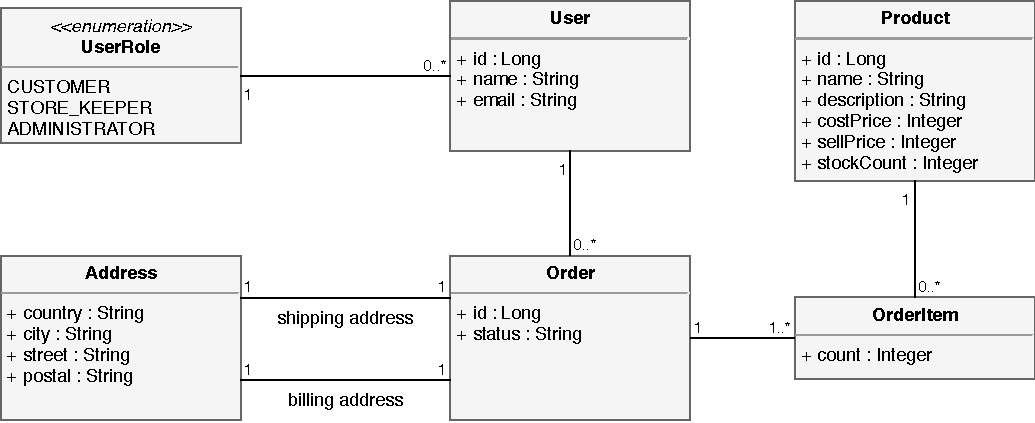
\includegraphics[keepaspectratio=true, width=0.9\linewidth]{figures/example-model.pdf}
    \caption{Doménový model ukázkového e-commerce systému}
    \label{fig:example-model}
\end{figure}

Tento model je využ\'{\i}ván v každé ze služeb. Nicméně, jednotlivé služby využívají
pouze jeho podmnožinu, kterou potřebují ke svoj\'{\i} práci.

\subsection{Byznysová pravidla a kontexty}

V tabulce~\ref{tbl:business-rules} je v\'yčet všech byznysov\'ych pravidel, která byla
vymodelována pro ukázkovou aplikaci. V tabulce kromě identifikátoru a popisu byznysového pravidla
vid\'{\i}me, na které užitné př\'{\i}pady se pravidlo aplikuje, a jak\'y je typ pravidla
(\textit{pre} pro precondition, \textit{post} pro post-condition).

\begin{table}
    \centering
    \begin{tabular}{ l l l r }
        \hline
        \textbf{\#} & \textbf{Use-cases} & \textbf{Pravidlo} & \textbf{Typ} \\ \hline \hline
        \textbf{BR01} & UC01 & Uživatel nesm\'{\i} b\'yt přihlášen\'y & pre \\ \hline
        \textbf{BR02} & UC02, UC03 & \makecell[l]{Uživatel nesm\'{\i} zobrazovat ani manipulovat \\ s produkty, které nejsou aktivn\'{\i}} & post \\ \hline
        \textbf{BR03} & UC02 až UC04 & \makecell[l]{Uživatel nesm\'{\i} u produktu vidět nákupn\'{\i} cenu, \\ pouze v\'yslednou cenu} & post \\ \hline
        \textbf{BR04} & UC04 & \makecell[l]{Zákazník mus\'{\i} řádně vyplnit doručovac\'{\i} \\ adresu (č.p., ulice, město, PSČ, stát)} & pre \\ \hline
        \textbf{BR05} & UC04, UC13 & \makecell[l]{Zákazník mus\'{\i} řádně vyplnit fakturačn\'{\i} \\ adresu (č.p., ulice, město, PSČ, stát)} & pre \\ \hline
        \textbf{BR06} & UC01, UC04, UC11 & Uživatel mus\'{\i} m\'{\i}t vyplněnou emailovou adresu & pre \\ \hline
        \textbf{BR07} & UC03 & \makecell[l]{Nákupní košík může obsahovat maximálně \\ 10 položek} & pre \\ \hline
        \textbf{BR08} & UC04 & \makecell[l]{Položky objednávky mus\'{\i} m\'{\i}t počet kusů menš\'{\i}, \\ než je aktuáln\'{\i} stav skladov\'ych zásob produktu} & pre \\ \hline
        \textbf{BR09} & UC04 & \makecell[l]{Stát mus\'{\i} b\'yt v seznamu zem\'{\i}, \\ do kter\'ych firma doručuje} & pre \\ \hline
        \textbf{BR10} & UC04 & Zákazn\'{\i}k mus\'{\i} b\'yt přihlášen & pre \\ \hline
        \textbf{BR11} & UC05 až UC08 & \makecell[l]{Skladn\'{\i}k mus\'{\i} b\'yt do systému přihlášen \\ a m\'{\i}t roli "Skladn\'{\i}k"} & pre \\ \hline
        \textbf{BR12} & UC02 & \makecell[l]{Skladn\'{\i}k u produktu nesm\'{\i} vidět nákupn\'{\i} cenu, \\ pouze v\'yslednou cenu} & post \\ \hline
        \textbf{BR13} & UC05 & Produkt mus\'{\i} m\'{\i}t jméno s délkou >5 & pre \\ \hline
        \textbf{BR14} & UC06 & \makecell[l]{Stav zásob produktů mus\'{\i} b\'yt č\'{\i}slo větš\'{\i} nebo \\ rovno 0} & pre \\ \hline
        \textbf{BR15} & UC08 & \makecell[l]{Stav objednávky mus\'{\i} b\'yt pouze "přijato", \\ "expedováno" a "doručeno"} & pre \\ \hline
        \textbf{BR16} & UC09 až UC13 & \makecell[l]{Administrátor mus\'{\i} b\'yt do systému přihlášen \\ a m\'{\i}t roli "Administrátor"} & pre \\ \hline
        \textbf{BR17} & UC10 & \makecell[l]{V\'ysledná cena produktu mus\'{\i} b\'yt větš\'{\i} \\ než jeho nákupn\'{\i} cena} & pre \\ \hline
        \textbf{BR18} & UC11 & Skladn\'{\i}k mus\'{\i} m\'{\i}t jméno delš\'{\i} než 2 znaky & pre \\ \hline
        \textbf{BR19} & UC12 & Smazaný uživatel nesmí být administrátor & pre \\ \hline
        \hline
    \end{tabular}
    \caption{Byznysová pravidla ukázkového e-commerce systému}
    \label{tbl:business-rules}
\end{table}

Dále jsou v tabulce~\ref{tbl:business-contexts} vypsány všechny byznysové kontexty v ukázkové aplikaci.
Některé z nich jsou konkrétn\'{\i} a jsou namapovány na jeden nebo v\'{\i}ce \gls{UC},
jiné jsou abstraktn\'{\i} a ostatn\'{\i} kontexty od nich dědí a sdílejí jejich byznysová pravidla.
Prefixy byly vybrány na základě byznysové domény, ke které se kontext vztahuje, stejně jako
jsou podle domén děleny i jednotlivé služby systému.

\begin{table}
    \centering
    \begin{tabular*}{\textwidth}{ l c l }
        \hline
        \textbf{Identifikátor} & \textbf{Use-cases} & \textbf{Byznysová pravidla} \\ \hline \hline
        \textbf{auth.adminLoggedIn} & - & BR16 \\ \hline
        \textbf{auth.employeeLoggedIn} & - & BR11 \\ \hline
        \textbf{auth.userLoggedIn} & - & BR10 \\ \hline
        \textbf{billing.correctAddress} & - & BR05 \\ \hline
        \textbf{billing.createInvoice} & UC13 & BR05 \\ \hline
        \textbf{order.addToShippingCart} & UC03 & BR02, BR07, BR08, BR10 \\ \hline
        \textbf{order.changeStatus} & UC08 & \makecell[l]{BR04, BR05, BR06, BR08, BR09, BR11, \\ BR15} \\ \hline
        \textbf{order.create} & UC04 & \makecell[l]{BR03, BR04, BR05, BR06, BR07, BR08, \\ BR09, BR10, BR15} \\ \hline
        \textbf{order.listAll} & UC07, UC09 & BR11 \\ \hline
        \textbf{order.valid} & - & BR04, BR05, BR06, BR09, BR15 \\ \hline
        \textbf{product.changePrice} & UC10 & BR16, BR17 \\ \hline
        \textbf{product.changeStock} & UC06 & BR08, BR11, BR14 \\ \hline
        \textbf{product.create} & UC05 & BR10, BR11, BR13, BR14 \\ \hline
        \textbf{product.detail} & UC02 & BR02, BR03, BR10, BR12 \\ \hline
        \textbf{product.hidden} & - & BR02 \\ \hline
        \textbf{product.listAll} & UC02 & BR02, BR03, BR12 \\ \hline
        \textbf{shipping.correctAddress} & - & BR04, BR09 \\ \hline
        \textbf{user.createCustomer} & UC01 & BR01, BR06 \\ \hline
        \textbf{user.createEmployee} & UC11 & BR06, BR16, BR18 \\ \hline
        \textbf{user.delete} & UC12 & BR16, BR19 \\ \hline
        \textbf{user.validEmail} & - & BR06 \\ \hline
        \hline
    \end{tabular*}
    \caption{Byznysové kontexty ukázkového e-commerce systému}
    \label{tbl:business-contexts}
\end{table}

Na obrázku~\ref{fig:example-system-context-hirearchy} je vizualizována
hierarchie byznysov\'ych kontextů v ukázkovém systému, jejich vazba na \gls{UC}
a také byznysová pravidla, která se v kontextech aplikuj\'{\i}.

\subsection{Služby}

Na obrázku~\ref{fig:example-system} jsou zobrazeny komponenty systému a jejich vzájemné závislosti.
Pro ověřen\'{\i} schopnosti podporovat v\'{\i}ce platforem byly pro implementaci systému využity
jazyky Java, Python a JavaScript v kombinaci s běhov\'ym prostřed\'{\i}m Node.js.
Komunikace služeb prob\'{\i}há pomoc\'{\i} \gls{REST} \gls{API} využ\'{\i}vaj\'{\i}c\'{\i} formát \gls{JSON}.
Specifikace jednotliv\'ych rozhran\'{\i} služeb nen\'{\i} pro tuto kapitolu podstatná, a proto se
j\'{\i} text dále nevěnuje. Pro demonstrativn\'{\i} účely byly s\'{\i}ťové adresy nastaveny př\'{\i}mo v kódu jednotliv\'ych
služeb. Nicméně, navržen\'y framework nevynucuje tento př\'{\i}stup, a tud\'{\i}ž by bylo možné komplexnější
způsob \textit{service discovery} do systému integrovat.

\begin{figure}
    \centering
    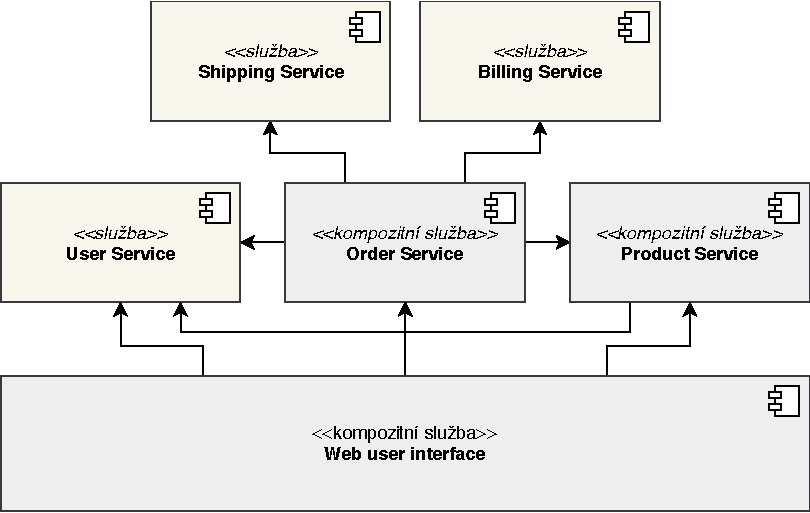
\includegraphics[keepaspectratio=true, width=0.8\linewidth]{figures/example-system.pdf}
    \caption{Komponenty ukázkového e-commerce systému}
    \label{fig:example-system}
\end{figure}

\paragraph{Billing service}

Služba \textit{Billing service} má na starosti funkcionalitu t\'ykaj\'{\i}c\'{\i} se fakturace objednávek
a byla implementována v jazyce Java s použit\'{\i}m frameworku Spring Boot\footnote{\url{https://projects.spring.io/spring-boot/}}.

\paragraph{Order service}

Kompozitn\'{\i} služba \textit{Order service} slouž\'{\i}c\'{\i} pro vytvářen\'{\i} a správu objednávek
byla implementována v jazyce Java a jej\'{\i} \gls{API} bylo sestaveno za použit\'{\i} frameworku Spring
Boot, jak je ukázáno ve zdrojovém kódu~\ref{lst:order-service-springboot}, kde
je ukázka obsluhy požadavků na v\'ypis zbož\'{\i} v koš\'{\i}ku uživatele.

\lstinputlisting[
caption={Ukázka využit\'{\i} frameworku Spring Boot pro účely Order service},
label={lst:order-service-springboot},
language=Java,
%frame=single,
]
{code/order_service.java}

\paragraph{Product service}

Služba \textit{Product service} realizuje \gls{UC} t\'ykaj\'{\i}c\'{\i} se
prohl\'{\i}žen\'{\i} a administrac\'{\i} nab\'{\i}zen\'ych
produktů a jejich skladov\'ych zásob. Služba byla implementována v jazyce Python.
Pro vytvořen\'{\i} \gls{REST} \gls{API} služby byl využit
light-weight framework \textit{Flask}\footnote{\url{http://flask.pocoo.org/}}.
Ve zdrojovém kódu~\ref{lst:product-service-flask} je znázorněno použit\'{\i}
tohoto frameworku pro obsluhu požadavku na v\'ypis všech produktů.

\lstinputlisting[
caption={Ukázka využit\'{\i} frameworku Flask pro účely Product service},
label={lst:product-service-flask},
language=Python,
%frame=single,
]
{code/product_service.py}

\paragraph{Shipping service}

Služba \textit{Shipping service} má na starosti funkcionalitu t\'ykaj\'{\i}c\'{\i} se odes\'{\i}lán\'{\i} objednávek
a byla implementována v jazyce Java s použit\'{\i}m frameworku Spring Boot.

\paragraph{User service}

Služba \textit{User service} realizuj\'{\i}c\'{\i} funkcionalitu t\'ykaj\'{\i}c\'{\i} se uživatelsk\'ych účtů byla
implementována v jazyce JavaScript na platformě Node.js s použit\'{\i}m
frameworku Express\footnote{\url{https://expressjs.com/}}. Ve zdrojovém kódu~\ref{lst:user-service-expressjs}
je ukázka mapován\'{\i} controllerů na \gls{URL} \code{/users} a různé metody protokolu \gls{HTTP}.

\lstinputlisting[
caption={Ukázka využit\'{\i} frameworku Express.js pro účely User service},
label={lst:user-service-expressjs},
language=JavaScript,
%frame=single,
]
{code/user_service.js}

\paragraph{Webové uživatelské rozhran\'{\i}}

Služba, která slouž\'{\i} uživatelům ukázkového systému jako webové uživatelské
rozhran\'{\i}, byla implementována v jazyce Java s použit\'{\i}m frameworku Spring Boot.
Na sn\'{\i}mku~\ref{fig:example-screenshot} je vidět UI ukázkového systému,
konkrétně informován\'{\i} uživatele o tom, že se nepodařilo přidat produkt
do koš\'{\i}ku, protože bylo porušeno byznysové pravidlo – koš\'{\i}k nesm\'{\i} obsahovat
v\'{\i}ce než 10 položek.

\paragraph{Centráln\'{\i} správa byznysov\'ych pravidel}

Do ukázkového systému byl nasazen také systém pro centráln\'{\i} správu byznysov\'ych kontextů,
kter\'y je popsan\'y v sekci~\ref{sec:central-administration}. Systém byl napojen na všechny
služby systému, kromě webového \gls{UI}, a bylo úspěšně demonstrováno, že lze za běhu systému
dynamicky upravovat byznysové kontexty, resp. jejich byznysová pravidla.

\paragraph{Běhové prostřed\'{\i} služeb}
Pro jednoduché spuštěn\'{\i} celého ukázkového systému byla využita technologie
Docker~\cite{merkel2014docker}, která umožňuje vytvořit virtuáln\'{\i} běhové prostřed\'{\i}
pro aplikaci pomoc\'{\i} kontejnerizace využ\'{\i}vaj\'{\i}c\'{\i} virtualizaci nad operačn\'{\i}m systémem.
Uživatel si nadefinuje tzv. \textit{image}, kter\'y se skládá z jednotliv\'ych vrstev.
Základn\'{\i} vrstvou je operačn\'{\i} systém, dalš\'{\i}mi mohou b\'yt jednotlivé knihovny instalované do systému.
%Př\'{\i}klad definice image pomoc\'{\i} technologie Docker je znázorněn ve zdrojovém
%kódu~\ref{lst:docker-image}. Konkrétně se jedná o definici image, kter\'y
%rozšiřuje oficiáln\'{\i} image \code{library/node:9.11.1}\footnote{\url{https://hub.docker.com/\_/node/}}
%stavěj\'{\i}c\'{\i} nad operačn\'{\i}m systémem \textit{Linux}\footnote{\url{https://www.linuxfoundation.org/projects/linux/}},
%a přidává vrstvy s prototypem knihovny pro platformu Node.js.

%\lstinputlisting[
%caption={Ukázka zápisu Docker image obsahuj\'{\i}c\'{\i} knihovnu pro platformu Node.js},
%label={lst:docker-image},
%language=Dockerfile,
%%frame=single,
%]
%{code/dockerfile_nodejs.txt}

\paragraph{Spouštěn\'{\i} služeb}
Pro samotné spuštěn\'{\i} byla využita funkce \textit{Docker Compose}, která umožňuje
definovat a spouštět aplikace s více kontejnery. Ve zdrojovém kódu~\ref{lst:docker-compose}
je příklad zápisu Order service. Pro jej\'{\i} image je použit \code{filipklimes-diploma/example-order-service}.
V sekci \code{ports} je deklarováno, že služba má m\'{\i}t z vnějšku př\'{\i}stupn\'y port \code{5501}, na kterém poskytuje své
\gls{REST} \gls{API}, a port \code{5551}, na kterém poskytuje své gRPC \gls{API} pro sd\'{\i}lené byznysov\'ych kontextů.
V sekci \code{links} je deklarováno, že pro kontejner, ve kterém Order Service poběž\'{\i}, maj\'{\i} b\'yt na s\'{\i}ti
př\'{\i}stupné služby \code{product}, \code{user}, \code{billing} a \code{shipping}. Vše je popsáno ve formátu \gls{YAML},
kter\'y je vhodný pro konfiguračn\'{\i} soubory díky jeho snadné čitelnosti pro člověka a jednoduchému použ\'{\i}ván\'{\i}.

\lstinputlisting[
caption={Ukázka zápisu aplikace s více kontejnery pro Docker Compose},
label={lst:docker-compose},
language=Yaml,
%frame=single,
]
{code/docker_compose.yml}

\section{Srovnán\'{\i} s konvenčn\'{\i}m př\'{\i}stupem}

%\goal{Ukázka na konkrétn\'{\i}m př\'{\i}kladě}
Z tabulky~\ref{tbl:business-contexts} plyne, že čtrnáct z devatenácti byznysových pravidel je využito ve více
byznysových kontextech a devět pravidel je sdíleno mezi v\'{\i}ce službami. V tabulce~\ref{tbl:duplication}
je přehledně shrnuto, která pravidla jsou využ\'{\i}vána ve kter\'ych službách. Při použit\'{\i} konvenčn\'{\i}ho př\'{\i}stupu
by tato pravidla bylo nutné implementovat alespoň jednou pro každou ze služeb, za předpokladu, že by nedocházelo k duplikac\'{\i}m
ve službách samotn\'ych. Manuáln\'{\i} duplikace nav\'{\i}c přináš\'{\i} nutnost synchronizovat podobu pravidla
při každém změnovém ř\'{\i}zen\'{\i}, což zvyšuje náklady na v\'yvoj a riziko lidské chyby.

\begin{table}
    \centering
    \begin{tabularx}{\textwidth}{ l X | l X }
        \hline
        \textbf{\#} & \textbf{Použito ve službách} & \textbf{\#} & \textbf{Použito ve službách} \\ \hline \hline
        \textbf{BR01} & user & \textbf{BR11} & auth, order, product \\
        \textbf{BR02} & order, product & \textbf{BR12} & product \\
        \textbf{BR03} & order, product & \textbf{BR13} & product \\
        \textbf{BR04} & order, shipping & \textbf{BR14} & product \\
        \textbf{BR05} & billing, order & \textbf{BR15} & order \\
        \textbf{BR06} & order, user & \textbf{BR16} & (auth), product, user \\
        \textbf{BR07} & order & \textbf{BR17} & product \\
        \textbf{BR08} & order & \textbf{BR18} & user \\
        \textbf{BR09} & order, shipping & \textbf{BR19} & user \\
        \textbf{BR10} & (auth), order, product & \\
        \hline
    \end{tabularx}
    \caption{Využit\'{\i} byznysov\'ych pravidel ve službách ukázkového systému}
    \label{tbl:duplication}
\end{table}

%\goal{V\'yhody frameworku}
D\'{\i}ky použit\'{\i} navrženého frameworku je však možné každé pravidlo nadefinovat na jednom místě
a framework se postará o jeho automatickou integraci do všech částí systému, kde má být aplikováno.
To umožňuje byznysová pravidla, resp. kontexty, spravovat pomoc\'{\i} nástroje pro
centráln\'{\i} správu, kter\'y je součást\'{\i} navrženého frameworku. Z toho vypl\'yvá
sn\'{\i}žen\'{\i} nároků na v\'yvoj a sn\'{\i}žené riziko lidské chyby.

%\goal{Nev\'yhody použit\'{\i}}
Jako nev\'yhodu použit\'{\i} frameworku lze považovat počátečn\'{\i} investici v podobě integrace knihoven do služeb systému.
a cena popisu byznysov\'ych pravidel v \gls{DSL}, kter\'y se musej\'{\i} v\'yvojáři systému naučit nav\'{\i}c
oproti programovac\'{\i}mu jazyku, ve kterém popisuj\'{\i} služby. Tento jazyk však mohou používat i doménoví experti, a tak
ulehčit práci vývojářů. Framework také není vhodné nasazovat v systémech, jejichž doména nemá tendenci sdílet byznysová pravidla.

%\goal{Závěr}
Navržen\'y framework tedy oproti konvenčn\'{\i}mu př\'{\i}stupu nab\'{\i}z\'{\i} možnost z\'{\i}skat dlouhodobě
nižš\'{\i} náklady na v\'yvoj za cenu počátečn\'{\i} investice. D\'{\i}ky provedené
př\'{\i}padové studii bylo ukázáno, že v \gls{SOA} lze efektivně řešit sdílení byznysov\'ych pravidel
navržen\'ym způsobem.

\section{Shrnut\'{\i}}

Tato kapitola popisuje, jak\'ym způsobem byly testovány prototypy knihoven
pro platformy jazyků Java a Python a pro platformu Node.js. Dále kapitola
specifikuje ukázkový systém, na kterém byla
provedena demonstrace použit\'{\i} frameworku, a popisuje jeho implementaci.
Tím bylo otestováno, že navržen\'y framework je funkčn\'{\i},
splňuje požadavky identifikované v sekci~\ref{sec:implementation-requirements}
a prokazuje reálné snížení manuální duplikace byznysových pravidel oproti
konvenčn\'{\i}mu př\'{\i}stupu k návrhu a implementaci softwarov\'ych systému.
